\PassOptionsToPackage{dvipsnames}{xcolor}
%\documentclass[amsmath,table,sans,amsfonts, handout]{beamer}
\documentclass[amsmath,table,sans,amsfonts]{beamer}
\usepackage[T1]{fontenc}
%%\usepackage{beamerthemeshadow}
%%\usepackage[headheight=1pt,footheight=10pt]{beamerthemeboxes}
%%\addfootboxtemplate{\color{structure!80}}{\color{white}\tiny \hfill Karl Svozil (TU Vienna)\hfill}
%%\addfootboxtemplate{\color{structure!65}}{\color{white}\tiny \hfill mur.sat \hfill}
%%\addfootboxtemplate{\color{structure!50}}{\color{white}\tiny \hfill Graz, 2010-12-11\hfill}
%\usepackage[dark]{beamerthemesidebar}
%\usepackage[headheight=24pt,footheight=12pt]{beamerthemesplit}
%\usepackage{beamerthemesplit}
%\usepackage[bar]{beamerthemetree}
\usepackage{graphicx}

%Global Background must be put in preamble
{%
%\usebackgroundtemplate%      \includegraphics[width=\paperwidth,height=\paperheight]{HaK-Urkaos-da}%
}
 \setbeamercolor{background canvas}{bg=black}

\usepackage{eepic}
%\usepackage[usenames]{color}
%\newcommand{\Red}{\color{Red}}  %(VERY-Approx.PANTONE-RED)
%\newcommand{\Green}{\color{Green}}  %(VERY-Approx.PANTONE-GREEN)


%\RequirePackage[german]{babel}
%\selectlanguage{german}
%\RequirePackage[isolatin]{inputenc}

%\pgfdeclareimage[height=0.5cm]{logo}{tu-logo}
%\logo{\pgfuseimage{logo}}
\beamertemplatetriangleitem
%\beamertemplateballitem

\beamerboxesdeclarecolorscheme{alert}{red}{red!15!averagebackgroundcolor}
%\begin{beamerboxesrounded}[scheme=alert,shadow=true]{}
%\end{beamerboxesrounded}

%\beamersetaveragebackground{yellow!10}

%\beamertemplatecircleminiframe

\newtheorem{question}{Question}
\newtheorem{conjecture}[question]{Principle}
\newtheorem{challenge}[question]{Challenge}

\usepackage{tikz}
\usetikzlibrary{calc,decorations.pathreplacing,decorations.markings}




\definecolor{orange(webcolor)}{rgb}{1.0, 0.65, 0.0}
\setbeamercolor{normal text}{fg=white}
\setbeamercolor{structure}{fg=orange}




\begin{document}




\title{\bf \color{white} {Value (in)definiteness and contextuality}}
\subtitle{ \color{white} {\footnotesize http://tph.tuwien.ac.at/$\sim$svozil/publ/2018-Svozil-Prague2018-pres.pdf
%\\
%Nature-Springer, in press 2017; drafts on demand
}}
\author{{Karl Svozil}}
\institute{{ITP/Vienna University of Technology, Austria\\
svozil@tuwien.ac.at
}
%{\tiny Disclaimer: Die hier vertretenen Meinungen des Autors verstehen sich als Diskussionsbeitr�ge und decken sich nicht notwendigerweise mit den Positionen der Technischen Universit�t Wien oder deren Vertreter.}
}
\date{\textcolor{white!100}{Prague, Czech Republic, May 21st, 2018}}

\maketitle

% \frame{
% \frametitle{}
%
% }




 \frame{
 \frametitle{\color{orange!100}Some questions one could ask, and answers one might expect}

\begin{itemize}
%\pause
\item
Does a(n empirical) structure of propositions (logic) uniquely induce a probability?  No!

\item
What kind of non-Boolean (non-classical) structure of propositions can one imagine?
\begin{itemize}
\item
Partition logic (Svozil 1993, Dvure{\v{c}}enskij, Pulmannov{\'{a}}{\&}Svozil, 1995); models include
\begin{itemize}
\item
Wright's generalized urn model as well as  (Wright, 1978, 1990)
\item
Moore's finite automaton state identification problem (Moore, Svozil 1993, Svozil{\&}Schaller, 1995,1996).
\end{itemize}
\item
quantum logic (Hilbert lattices)

\item
general logics constructed by the pasting of Boolean subalgebras (contexts, blocks)
\end{itemize}

\item
What criteria/axioms to assume for probabilities?
Classical Kolmogorov's probability theory for classical bits \& pieces or blocks.
``Stitching'' or ``pasting'' of these blocks.
Eg, Gleason-type frame functions on quantum contexts: additivity of mutually exclusive events, totally  (im)probable events have probability 0 and 1, respectively.


\end{itemize}



 }






\frame{
\frametitle{\color{orange!100}(Geometric) Strategies to classical probabilities
}

\begin{itemize}
%\pause
\item
Froissart (1981), Pitowsky (1986), Tsirelson (1993): geometric interpretation of probability distributions
as the surface of a convex polytope ``spanned''
by vertices aka ``mutually exclusive extreme cases.''


\begin{itemize}
%\pause
\item
The vertices are encoded by two-valued states on the logic.

\item
The Bell-type face (in)equalities indicating ``inside-outside relations'' are
very similar to Boole's ``conditions of possible experience'' (1854,1862).
The  {\em hull problem} of finding these faces is NP-complete in the number of vertices.
\end{itemize}

\item
Wright (1978,1990): Quasiclassical probabilities are in the convex hull of the dispersion-free two-valued states (aka classical truth assignments).



\end{itemize}
}

\begin{frame}[fragile]{Heuristic use of the terms value indefiniteness and contextuality}


Heuristically, a collection of observables (hypothetical propositions) can be called {\em contextual} if (in order of severe deviation from classicality) it
\begin{itemize}
\item
``somehow'' is not classical; eg. exhibits complementarity (non-distributivity);
\item
has no (quasi)classical probability interpretation in terms of the convex hull of the  (Kochen{\&}Specker 1967, Theorem~0: {\color{red}separating}) set of classical truth assignments;
\item
is partial (unless inconsistent) and thus value indefinite (Gleason 1957, Zierler{\&}Schlessinger 1965, Kochen{\&}Specker 1967, Pitowsky  1998, ACCS, ACS, 2012-2015).
\end{itemize}

\end{frame}

\begin{frame}[fragile]{Trigger warning}


The term contextuality has been used by the realist John Bell to enforce value definiteness on intertwined collections of observables
(grouped into maximal classical subalgebras called ``contexts,'' ``cliques'' or ``blocks'') at the price of their dependency on the
measurement context -- thereby effectively discarding the assumption of an ``isolated'' observable (from whatever is effectively co-measured alongside of it).
This is in contrast to the quantum (logical) formalism, in particular to elementary propositions identified with perpendicular projection operators.

Thus the current wide use of the term contextuality is often-times confusing and distractive:
many researchers using the term would not like it to imply realism and context dependence of quantum observables.

\end{frame}



\begin{frame}[fragile]{Example I: Pentagon logic}

\begin{tabular}{cc}
\begin{tabular}{c}
\\
%TexCad Options
%\grade{\off}
%\emlines{\off}
%\beziermacro{\off}
%\reduce{\on}
%\snapping{\off}
%\quality{0.20}
%\graddiff{0.01}
%\snapasp{1}
%\zoom{1.00}
\unitlength 0.17mm
%\thicklines %\linethickness{1pt}
\allinethickness{2.1pt}
\begin{picture}(230,200)(-110,-100)
%\emline(31,-95.25)(100,0)
\multiput(31,-95.25)(.033724340176,.046554252199){2046}{\color{cyan}\line(0,1){.046554252199}}
%\end
%\emline(100,0)(31,95)
\multiput(100,0)(-.033724340176,.046432062561){2046}{\color{magenta}\line(0,1){.046432062561}}
%\end
%\emline(31,95)(-81,58.75)
\multiput(31,95)(-.10418604651,-.03372093023){1075}{\color{blue}\line(-1,0){.10418604651}}
%\end
\put(-81,58.75){\color{red}\line(0,-1){117.75}}
%\emline(-81,-59)(30.75,-95.5)
\multiput(-81,-59)(.10328096118,-.03373382625){1082}{\color{green}\line(1,0){.10328096118}}
%\end
%
\put( 30.9017 , 95.1057){\color{magenta}\circle{15.00}}
\put( 30.9017 , 95.1057){\color{blue}\circle{6}} %1
\put( 30.9017 , 95.1057){\color{blue}\circle{1}} %1
\put( 55.9017 , 95.1057){\makebox(0,0)[cc]{$1$}}
%
\put( 65.4509,47.5529){\color{magenta}\circle{9}}  %2
\put( 90.4509,47.5529){\makebox(0,0)[cc]{$2$}}
%
%
\put(100,0){\color{cyan}\circle{15.00}}
\put(100,0){\color{magenta}\circle{6}}    %3
\put(100,0){\color{magenta}\circle{1}}    %3
\put(120,0){\makebox(0,0)[cc]{$3$}}
%
\put( 65.4509,-47.5529){\color{cyan}\circle{9}}  %4
\put( 90.4509,-47.5529){\makebox(0,0)[cc]{$4$}}
%
\put( 30.9017 , -95.1057){\color{green}\circle{15.00}}
\put( 30.9017 , -95.1057){\color{cyan}\circle{6}}  %5
\put( 30.9017 , -95.1057){\color{cyan}\circle{1}}  %5
\put( 55.9017 , -95.1057){\makebox(0,0)[cc]{$5$}}
%
\put( -25,-76.9421){\color{green}\circle{9}}         %6
\put( -40,-90.9421){\makebox(0,0)[cc]{$6$}}
%
\put( -80.9017 , -58.7785){\color{red}\circle{15.00}}
\put( -80.9017 , -58.7785){\color{green}\circle{6}}   %7
\put( -80.9017 , -58.7785){\color{green}\circle{1}}   %7
\put( -105.9017 , -58.7785){\makebox(0,0)[cc]{$7$}}
%
\put(-80.9017,0){\color{red}\circle{9}}           %8
\put(-105.9017,0){\makebox(0,0)[cc]{$8$}}
%
\put(-80.9017 , 58.7785){\color{blue}\circle{15}}
\put(-80.9017 , 58.7785){\color{red}\circle{6}}     %9
\put(-80.9017 , 58.7785){\color{red}\circle{1}}     %9
\put(-105.9017 , 58.7785){\makebox(0,0)[cc]{$9$}}
%
\put( -25,76.9421){\color{blue}\circle{9}}         %10
\put( -40,90.9421){\makebox(0,0)[cc]{${10}$}}
\end{picture}
\end{tabular}
&
{\footnotesize
\setlength{\tabcolsep}{2pt}
\renewcommand{\arraystretch}{1}
 \begin{tabular}{ccccccccccc}
\#
&
$1$&
$2$&
$3$&
$4$&
$5$&
$6$&
$7$&
$8$&
$9$&
${10}$
\\
\hline
$v_1$&1&  0&  0& 1&  0& 1&  0& 1&  0&  0 \\
$v_2$&1&  0&  0&  0& 1&  0&  0& 1&  0&  0\\
$v_3$&1&  0&  0& 1&  0&  0& 1&  0&  0&  0\\
$v_4$&0&  0& 1&  0&  0& 1&  0& 1&  0& 1\\
$v_5$&0&  0& 1&  0&  0&  0& 1&  0&  0& 1\\
$v_6$&0&  0& 1&  0&  0& 1&  0&  0& 1&  0\\
$v_7$&0& 1&  0&  0& 1&  0&  0& 1&  0& 1\\
$v_8$&0& 1&  0&  0& 1&  0&  0&  0& 1&  0\\
$v_9$&0& 1&  0& 1&  0&  0& 1&  0&  0& 1\\
$v_{10}$&0& 1&  0& 1&  0& 1&  0&  0& 1&  0\\
$v_{11}$&0& 1&  0& 1&  0& 1&  0& 1&  0& 1 \\
\hline
$v_e$&$\frac{1}{2}$& 0&  $\frac{1}{2}$& 0&  $\frac{1}{2}$& 0&  $\frac{1}{2}$& 0&  $\frac{1}{2}$& 0
 \end{tabular}
}
\end{tabular}


\end{frame}





\begin{frame}[fragile]{Example I: two-valued states on the pentagon logic (Wright, 1978)}

 \begin{center}
\begin{tabular}{cccc}
%TexCad Options
%\grade{\off}
%\emlines{\off}
%\beziermacro{\off}
%\reduce{\on}
%\snapping{\off}
%\quality{0.20}
%\graddiff{0.01}
%\snapasp{1}
%\zoom{1.00}
\unitlength 0.08mm
%\thicklines %\linethickness{1pt}
\allinethickness{1.5pt}
\begin{picture}(230,200)(-110,-100)
\put(0,0){\makebox(0,0)[cc]{\large $v_1$}}
%\emline(31,-95.25)(100,0)
\multiput(31,-95.25)(1.2,1.6565){58}{\color{cyan}\line(0,1){.1656521739}}
%\end
%\emline(100,0)(31,95)
\multiput(100,0)(-1.2,1.6522){58}{\color{magenta}\line(0,1){.1652173913}}
%\end
%\emline(31,95)(-81,58.75)
\multiput(31,95)(-3.69637,-1.19637){30}{\color{blue}\line(-1,0){.3696369637}}
%\end
%\put(-81,58.75){\color{red}\line(0,-1){117.75}}
\multiput(-81,59)(0,-2){60}{\color{red}\line(0,-1){0.33}}
%\emline(-81,-59)(30.75,-95.5)
\multiput(-81,-59)(3.664,-1.1967){31}{\color{green}\line(1,0){.3663934426}}
%\end
%
\put( 30.9017 , 95.1057){\circle{4}} %1
\put( 65.4509,-47.5529){\circle{4}}  %4
\put( -25,-76.9421){\circle{4}}         %6
\put(-80.9017,0){\circle{4}}           %8
\put( 30.9017 , 95.1057){\circle{10}} %1
\put( 65.4509,-47.5529){\circle{10}}  %4
\put( -25,-76.9421){\circle{10}}         %6
\put(-80.9017,0){\circle{10}}           %8
\put( 30.9017 , 95.1057){\circle{18}} %1
\put( 65.4509,-47.5529){\circle{18}}  %4
\put( -25,-76.9421){\circle{18}}         %6
\put(-80.9017,0){\circle{18}}           %8
\end{picture}
&
%TexCad Options
%\grade{\off}
%\emlines{\off}
%\beziermacro{\off}
%\reduce{\on}
%\snapping{\off}
%\quality{0.20}
%\graddiff{0.01}
%\snapasp{1}
%\zoom{1.00}
\unitlength 0.08mm
%\thicklines %\linethickness{1pt}
\allinethickness{1.5pt}
\begin{picture}(230,200)(-110,-100)
\put(0,0){\makebox(0,0)[cc]{\large $v_2$}}
%\emline(31,-95.25)(100,0)
\multiput(31,-95.25)(1.2,1.6565){58}{\color{cyan}\line(0,1){.1656521739}}
%\end
%\emline(100,0)(31,95)
\multiput(100,0)(-1.2,1.6522){58}{\color{magenta}\line(0,1){.1652173913}}
%\end
%\emline(31,95)(-81,58.75)
\multiput(31,95)(-3.69637,-1.19637){30}{\color{blue}\line(-1,0){.3696369637}}
%\end
\multiput(-81,59)(0,-2){60}{\color{red}\line(0,-1){0.33}}
%\emline(-81,-59)(30.75,-95.5)
\multiput(-81,-59)(3.664,-1.1967){31}{\color{green}\line(1,0){.3663934426}}
%\end
%
\put( 30.9017 , 95.1057){\circle{4}} %1
\put( 30.9017 , -95.1057){\circle{4}}  %5
\put(-80.9017,0){\circle{4}}           %8
\put( 30.9017 , 95.1057){\circle{10}} %1
\put( 30.9017 , -95.1057){\circle{10}}  %5
\put(-80.9017,0){\circle{10}}           %8
\put( 30.9017 , 95.1057){\circle{18}} %1
\put( 30.9017 , -95.1057){\circle{18}}  %5
\put(-80.9017,0){\circle{18}}           %8
\end{picture}
&
%TexCad Options
%\grade{\off}
%\emlines{\off}
%\beziermacro{\off}
%\reduce{\on}
%\snapping{\off}
%\quality{0.20}
%\graddiff{0.01}
%\snapasp{1}
%\zoom{1.00}
\unitlength 0.08mm
%\thicklines %\linethickness{1pt}
\allinethickness{1.5pt}
\begin{picture}(230,200)(-110,-100)
\put(0,0){\makebox(0,0)[cc]{\large $v_3$}}
%\emline(31,-95.25)(100,0)
\multiput(31,-95.25)(1.2,1.6565){58}{\color{cyan}\line(0,1){.1656521739}}
%\end
%\emline(100,0)(31,95)
\multiput(100,0)(-1.2,1.6522){58}{\color{magenta}\line(0,1){.1652173913}}
%\end
%\emline(31,95)(-81,58.75)
\multiput(31,95)(-3.69637,-1.19637){30}{\color{blue}\line(-1,0){.3696369637}}
%\end
\multiput(-81,59)(0,-2){60}{\color{red}\line(0,-1){0.33}}
%\emline(-81,-59)(30.75,-95.5)
\multiput(-81,-59)(3.664,-1.1967){31}{\color{green}\line(1,0){.3663934426}}
%\end
%
\put( 30.9017 , 95.1057){\circle{4}} %1
\put( 65.4509,-47.5529){\circle{4}}  %4
\put( -80.9017 , -58.7785){\circle{4}}   %7
\put( 30.9017 , 95.1057){\circle{10}} %1
\put( 65.4509,-47.5529){\circle{10}}  %4
\put( -80.9017 , -58.7785){\circle{10}}   %7
\put( 30.9017 , 95.1057){\circle{18}} %1
\put( 65.4509,-47.5529){\circle{18}}  %4
\put( -80.9017 , -58.7785){\circle{18}}   %7
\end{picture}
&
%TexCad Options
%\grade{\off}
%\emlines{\off}
%\beziermacro{\off}
%\reduce{\on}
%\snapping{\off}
%\quality{0.20}
%\graddiff{0.01}
%\snapasp{1}
%\zoom{1.00}
\unitlength 0.08mm
%\thicklines %\linethickness{1pt}
\allinethickness{1.5pt}
\begin{picture}(230,200)(-110,-100)
\put(0,0){\makebox(0,0)[cc]{\large $v_4$}}
%\emline(31,-95.25)(100,0)
\multiput(31,-95.25)(1.2,1.6565){58}{\color{cyan}\line(0,1){.1656521739}}
%\end
%\emline(100,0)(31,95)
\multiput(100,0)(-1.2,1.6522){58}{\color{magenta}\line(0,1){.1652173913}}
%\end
%\emline(31,95)(-81,58.75)
\multiput(31,95)(-3.69637,-1.19637){30}{\color{blue}\line(-1,0){.3696369637}}
%\end
\multiput(-81,59)(0,-2){60}{\color{red}\line(0,-1){0.33}}
%\emline(-81,-59)(30.75,-95.5)
\multiput(-81,-59)(3.664,-1.1967){31}{\color{green}\line(1,0){.3663934426}}
%\end
%
\put(100,0){\circle{4}}    %3
\put( -25,-76.9421){\circle{4}}         %6
\put(-80.9017,0){\circle{4}}           %8
\put( -25,76.9421){\circle{4}}         %10
\put(100,0){\circle{10}}    %3
\put( -25,-76.9421){\circle{10}}         %6
\put(-80.9017,0){\circle{10}}           %8
\put( -25,76.9421){\circle{10}}         %10
\put(100,0){\circle{18}}    %3
\put( -25,-76.9421){\circle{18}}         %6
\put(-80.9017,0){\circle{18}}           %8
\put( -25,76.9421){\circle{18}}         %10
\end{picture}
\\
%TexCad Options
%\grade{\off}
%\emlines{\off}
%\beziermacro{\off}
%\reduce{\on}
%\snapping{\off}
%\quality{0.20}
%\graddiff{0.01}
%\snapasp{1}
%\zoom{1.00}
\unitlength 0.08mm
%\thicklines %\linethickness{1pt}
\allinethickness{1.5pt}
\begin{picture}(230,200)(-110,-100)
\put(0,0){\makebox(0,0)[cc]{\large $v_5$}}
%\emline(31,-95.25)(100,0)
\multiput(31,-95.25)(1.2,1.6565){58}{\color{cyan}\line(0,1){.1656521739}}
%\end
%\emline(100,0)(31,95)
\multiput(100,0)(-1.2,1.6522){58}{\color{magenta}\line(0,1){.1652173913}}
%\end
%\emline(31,95)(-81,58.75)
\multiput(31,95)(-3.69637,-1.19637){30}{\color{blue}\line(-1,0){.3696369637}}
%\end
\multiput(-81,59)(0,-2){60}{\color{red}\line(0,-1){0.33}}
%\emline(-81,-59)(30.75,-95.5)
\multiput(-81,-59)(3.664,-1.1967){31}{\color{green}\line(1,0){.3663934426}}
%\end
%
\put(100,0){\circle{4}}    %3
\put( -80.9017 , -58.7785){\circle{4}}   %7
\put( -25,76.9421){\circle{4}}         %10
\put(100,0){\circle{10}}    %3
\put( -80.9017 , -58.7785){\circle{10}}   %7
\put( -25,76.9421){\circle{10}}         %10
\put(100,0){\circle{18}}    %3
\put( -80.9017 , -58.7785){\circle{18}}   %7
\put( -25,76.9421){\circle{18}}         %10
\end{picture}
&
%TexCad Options
%\grade{\off}
%\emlines{\off}
%\beziermacro{\off}
%\reduce{\on}
%\snapping{\off}
%\quality{0.20}
%\graddiff{0.01}
%\snapasp{1}
%\zoom{1.00}
\unitlength 0.08mm
%\thicklines %\linethickness{1pt}
\allinethickness{1.5pt}
\begin{picture}(230,200)(-110,-100)
\put(0,0){\makebox(0,0)[cc]{\large $v_6$}}
%\emline(31,-95.25)(100,0)
\multiput(31,-95.25)(1.2,1.6565){58}{\color{cyan}\line(0,1){.1656521739}}
%\end
%\emline(100,0)(31,95)
\multiput(100,0)(-1.2,1.6522){58}{\color{magenta}\line(0,1){.1652173913}}
%\end
%\emline(31,95)(-81,58.75)
\multiput(31,95)(-3.69637,-1.19637){30}{\color{blue}\line(-1,0){.3696369637}}
%\end
\multiput(-81,59)(0,-2){60}{\color{red}\line(0,-1){0.33}}
%\emline(-81,-59)(30.75,-95.5)
\multiput(-81,-59)(3.664,-1.1967){31}{\color{green}\line(1,0){.3663934426}}
%\end
%
\put(100,0){\circle{4}}    %3
\put( -25,-76.9421){\circle{4}}         %6
\put(-80.9017 , 58.7785){\circle{4}}     %9
\put(100,0){\circle{10}}    %3
\put( -25,-76.9421){\circle{10}}         %6
\put(-80.9017 , 58.7785){\circle{10}}     %9
\put(100,0){\circle{18}}    %3
\put( -25,-76.9421){\circle{18}}         %6
\put(-80.9017 , 58.7785){\circle{18}}     %9
\end{picture}
&
%TexCad Options
%\grade{\off}
%\emlines{\off}
%\beziermacro{\off}
%\reduce{\on}
%\snapping{\off}
%\quality{0.20}
%\graddiff{0.01}
%\snapasp{1}
%\zoom{1.00}
\unitlength 0.08mm
%\thicklines %\linethickness{1pt}
\allinethickness{1.5pt}
\begin{picture}(230,200)(-110,-100)
\put(0,0){\makebox(0,0)[cc]{\large $v_7$}}
%\emline(31,-95.25)(100,0)
\multiput(31,-95.25)(1.2,1.6565){58}{\color{cyan}\line(0,1){.1656521739}}
%\end
%\emline(100,0)(31,95)
\multiput(100,0)(-1.2,1.6522){58}{\color{magenta}\line(0,1){.1652173913}}
%\end
%\emline(31,95)(-81,58.75)
\multiput(31,95)(-3.69637,-1.19637){30}{\color{blue}\line(-1,0){.3696369637}}
%\end
\multiput(-81,59)(0,-2){60}{\color{red}\line(0,-1){0.33}}
%\emline(-81,-59)(30.75,-95.5)
\multiput(-81,-59)(3.664,-1.1967){31}{\color{green}\line(1,0){.3663934426}}
%\end
%
\put( 65.4509,47.5529){\circle{4}}  %2
\put( 30.9017 , -95.1057){\circle{4}}  %5
\put(-80.9017,0){\circle{4}}           %8
\put( -25,76.9421){\circle{4}}         %10
\put( 65.4509,47.5529){\circle{10}}  %2
\put( 30.9017 , -95.1057){\circle{10}}  %5
\put(-80.9017,0){\circle{10}}           %8
\put( -25,76.9421){\circle{10}}         %10
\put( 65.4509,47.5529){\circle{18}}  %2
\put( 30.9017 , -95.1057){\circle{18}}  %5
\put(-80.9017,0){\circle{18}}           %8
\put( -25,76.9421){\circle{18}}         %10
\end{picture}
&
%TexCad Options
%\grade{\off}
%\emlines{\off}
%\beziermacro{\off}
%\reduce{\on}
%\snapping{\off}
%\quality{0.20}
%\graddiff{0.01}
%\snapasp{1}
%\zoom{1.00}
\unitlength 0.08mm
%\thicklines %\linethickness{1pt}
\allinethickness{1.5pt}
\begin{picture}(230,200)(-110,-100)
\put(0,0){\makebox(0,0)[cc]{\large $v_8$}}
%\emline(31,-95.25)(100,0)
\multiput(31,-95.25)(1.2,1.6565){58}{\color{cyan}\line(0,1){.1656521739}}
%\end
%\emline(100,0)(31,95)
\multiput(100,0)(-1.2,1.6522){58}{\color{magenta}\line(0,1){.1652173913}}
%\end
%\emline(31,95)(-81,58.75)
\multiput(31,95)(-3.69637,-1.19637){30}{\color{blue}\line(-1,0){.3696369637}}
%\end
\multiput(-81,59)(0,-2){60}{\color{red}\line(0,-1){0.33}}
%\emline(-81,-59)(30.75,-95.5)
\multiput(-81,-59)(3.664,-1.1967){31}{\color{green}\line(1,0){.3663934426}}
%\end
%
\put( 65.4509,47.5529){\circle{4}}  %2
\put( 30.9017 , -95.1057){\circle{4}}  %5
\put(-80.9017 , 58.7785){\circle{4}}     %9
\put( 65.4509,47.5529){\circle{10}}  %2
\put( 30.9017 , -95.1057){\circle{10}}  %5
\put(-80.9017 , 58.7785){\circle{10}}     %9
\put( 65.4509,47.5529){\circle{18}}  %2
\put( 30.9017 , -95.1057){\circle{18}}  %5
\put(-80.9017 , 58.7785){\circle{18}}     %9
\end{picture}
\\
%TexCad Options
%\grade{\off}
%\emlines{\off}
%\beziermacro{\off}
%\reduce{\on}
%\snapping{\off}
%\quality{0.20}
%\graddiff{0.01}
%\snapasp{1}
%\zoom{1.00}
\unitlength 0.08mm
%\thicklines %\linethickness{1pt}
\allinethickness{1.5pt}
\begin{picture}(230,200)(-110,-100)
\put(0,0){\makebox(0,0)[cc]{\large $v_9$}}
%\emline(31,-95.25)(100,0)
\multiput(31,-95.25)(1.2,1.6565){58}{\color{cyan}\line(0,1){.1656521739}}
%\end
%\emline(100,0)(31,95)
\multiput(100,0)(-1.2,1.6522){58}{\color{magenta}\line(0,1){.1652173913}}
%\end
%\emline(31,95)(-81,58.75)
\multiput(31,95)(-3.69637,-1.19637){30}{\color{blue}\line(-1,0){.3696369637}}
%\end
\multiput(-81,59)(0,-2){60}{\color{red}\line(0,-1){0.33}}
%\emline(-81,-59)(30.75,-95.5)
\multiput(-81,-59)(3.664,-1.1967){31}{\color{green}\line(1,0){.3663934426}}
%\end
%
\put( 65.4509,47.5529){\circle{4}}  %2
\put( 65.4509,-47.5529){\circle{4}}  %4
\put( -80.9017 , -58.7785){\circle{4}}   %7
\put( -25,76.9421){\circle{4}}         %10
\put( 65.4509,47.5529){\circle{10}}  %2
\put( 65.4509,-47.5529){\circle{10}}  %4
\put( -80.9017 , -58.7785){\circle{10}}   %7
\put( -25,76.9421){\circle{10}}         %10
\put( 65.4509,47.5529){\circle{18}}  %2
\put( 65.4509,-47.5529){\circle{18}}  %4
\put( -80.9017 , -58.7785){\circle{18}}   %7
\put( -25,76.9421){\circle{18}}         %10
\end{picture}
&
%TexCad Options
%\grade{\off}
%\emlines{\off}
%\beziermacro{\off}
%\reduce{\on}
%\snapping{\off}
%\quality{0.20}
%\graddiff{0.01}
%\snapasp{1}
%\zoom{1.00}
\unitlength 0.08mm
%\thicklines %\linethickness{1pt}
\allinethickness{1.5pt}
\begin{picture}(230,200)(-110,-100)
\put(0,0){\makebox(0,0)[cc]{\large $v_{10}$}}
%\emline(31,-95.25)(100,0)
\multiput(31,-95.25)(1.2,1.6565){58}{\color{cyan}\line(0,1){.1656521739}}
%\end
%\emline(100,0)(31,95)
\multiput(100,0)(-1.2,1.6522){58}{\color{magenta}\line(0,1){.1652173913}}
%\end
%\emline(31,95)(-81,58.75)
\multiput(31,95)(-3.69637,-1.19637){30}{\color{blue}\line(-1,0){.3696369637}}
%\end
\multiput(-81,59)(0,-2){60}{\color{red}\line(0,-1){0.33}}
%\emline(-81,-59)(30.75,-95.5)
\multiput(-81,-59)(3.664,-1.1967){31}{\color{green}\line(1,0){.3663934426}}
%\end
%
\put( 65.4509,47.5529){\circle{4}}  %2
\put( 65.4509,-47.5529){\circle{4}}  %4
\put( -25,-76.9421){\circle{4}}         %6
\put(-80.9017 , 58.7785){\circle{4}}     %9
\put( 65.4509,47.5529){\circle{10}}  %2
\put( 65.4509,-47.5529){\circle{10}}  %4
\put( -25,-76.9421){\circle{10}}         %6
\put(-80.9017 , 58.7785){\circle{10}}     %9
\put( 65.4509,47.5529){\circle{18}}  %2
\put( 65.4509,-47.5529){\circle{18}}  %4
\put( -25,-76.9421){\circle{18}}         %6
\put(-80.9017 , 58.7785){\circle{18}}     %9
\end{picture}
%
&
%TexCad Options
%\grade{\off}
%\emlines{\off}
%\beziermacro{\off}
%\reduce{\on}
%\snapping{\off}
%\quality{0.20}
%\graddiff{0.01}
%\snapasp{1}
%\zoom{1.00}
\unitlength 0.08mm
%\thicklines %\linethickness{1pt}
\allinethickness{1.5pt}
\begin{picture}(230,200)(-110,-100)
\put(0,0){\makebox(0,0)[cc]{\large $v_{11}$}}
%\emline(31,-95.25)(100,0)
\multiput(31,-95.25)(1.2,1.6565){58}{\color{cyan}\line(0,1){.1656521739}}
%\end
%\emline(100,0)(31,95)
\multiput(100,0)(-1.2,1.6522){58}{\color{magenta}\line(0,1){.1652173913}}
%\end
%\emline(31,95)(-81,58.75)
\multiput(31,95)(-3.69637,-1.19637){30}{\color{blue}\line(-1,0){.3696369637}}
%\end
\multiput(-81,59)(0,-2){60}{\color{red}\line(0,-1){0.33}}
%\emline(-81,-59)(30.75,-95.5)
\multiput(-81,-59)(3.664,-1.1967){31}{\color{green}\line(1,0){.3663934426}}
%\end
%
\put( 65.4509,47.5529){\circle{4}}  %2
\put( 65.4509,-47.5529){\circle{4}}  %4
\put( -25,-76.9421){\circle{4}}         %6
\put(-80.9017,0){\circle{4}}           %8
\put( -25,76.9421){\circle{4}}         %10
\put( 65.4509,47.5529){\circle{10}}  %2
\put( 65.4509,-47.5529){\circle{10}}  %4
\put( -25,-76.9421){\circle{10}}         %6
\put(-80.9017,0){\circle{10}}           %8
\put( -25,76.9421){\circle{10}}         %10
\put( 65.4509,47.5529){\circle{18}}  %2
\put( 65.4509,-47.5529){\circle{18}}  %4
\put( -25,-76.9421){\circle{18}}         %6
\put(-80.9017,0){\circle{18}}           %8
\put( -25,76.9421){\circle{18}}         %10
\end{picture}
&
%TexCad Options
%\grade{\off}
%\emlines{\off}
%\beziermacro{\off}
%\reduce{\on}
%\snapping{\off}
%\quality{0.20}
%\graddiff{0.01}
%\snapasp{1}
%\zoom{1.00}
\unitlength 0.08mm
%\thicklines %\linethickness{1pt}
\allinethickness{1.5pt}
\begin{picture}(230,200)(-110,-100)
\put(0,0){\makebox(0,0)[cc]{\large $v_e$}}
%\emline(31,-95.25)(100,0)
\multiput(31,-95.25)(1.2,1.6565){58}{\color{cyan}\line(0,1){.1656521739}}
%\end
%\emline(100,0)(31,95)
\multiput(100,0)(-1.2,1.6522){58}{\color{magenta}\line(0,1){.1652173913}}
%\end
%\emline(31,95)(-81,58.75)
\multiput(31,95)(-3.69637,-1.19637){30}{\color{blue}\line(-1,0){.3696369637}}
%\end
\multiput(-81,59)(0,-2){60}{\color{red}\line(0,-1){0.33}}
%\emline(-81,-59)(30.75,-95.5)
\multiput(-81,-59)(3.664,-1.1967){31}{\color{green}\line(1,0){.3663934426}}
%\end
%
%
\put( 30.9017 , 95.1057){\color{orange}\circle{4}} %1
\put(100,0){\color{orange}\circle{4}}    %3
\put( 30.9017 , -95.1057){\color{orange}\circle{4}}  %5
\put( -80.9017 , -58.7785){\color{orange}\circle{4}}   %7
\put(-80.9017 , 58.7785){\color{orange}\circle{4}}     %9
\put( 30.9017 , 95.1057){\color{orange}\circle{10}} %1
\put(100,0){\color{orange}\circle{10}}    %3
\put( 30.9017 , -95.1057){\color{orange}\circle{10}}  %5
\put( -80.9017 , -58.7785){\color{orange}\circle{10}}   %7
\put(-80.9017 , 58.7785){\color{orange}\circle{10}}     %9
\put( 30.9017 , 95.1057){\color{orange}\circle{18}} %1
\put(100,0){\color{orange}\circle{18}}    %3
\put( 30.9017 , -95.1057){\color{orange}\circle{18}}  %5
\put( -80.9017 , -58.7785){\color{orange}\circle{18}}   %7
\put(-80.9017 , 58.7785){\color{orange}\circle{18}}     %9
\end{picture}
\end{tabular}
 \end{center}
\end{frame}



\begin{frame}[fragile]{Example I: Probabilities on partition logics from two-valued states on the pentagon logic -- with
$\lambda_i \ge 0$, $i=1,\ldots 11$, $\sum_{i=1}^{11} \lambda_i = 1$}

 \begin{center}
%TexCad Options
%\grade{\off}
%\emlines{\off}
%\beziermacro{\off}
%\reduce{\on}
%\snapping{\off}
%\quality{0.20}
%\graddiff{0.01}
%\snapasp{1}
%\zoom{1.00}
\unitlength 0.12mm
%\thicklines %\linethickness{1pt}
\allinethickness{2.1pt}
\begin{picture}(230,250)(-110,-115)
%\emline(31,-95.25)(100,0)
\multiput(31,-95.25)(.033724340176,.046554252199){2046}{\color{cyan}\line(0,1){.046554252199}}
%\end
%\emline(100,0)(31,95)
\multiput(100,0)(-.033724340176,.046432062561){2046}{\color{magenta}\line(0,1){.046432062561}}
%\end
%\emline(31,95)(-81,58.75)
\multiput(31,95)(-.10418604651,-.03372093023){1075}{\color{blue}\line(-1,0){.10418604651}}
%\end
\put(-81,58.75){\color{red}\line(0,-1){117.75}}
%\emline(-81,-59)(30.75,-95.5)
\multiput(-81,-59)(.10328096118,-.03373382625){1082}{\color{green}\line(1,0){.10328096118}}
%\end
%
\put( 30.9017 , 95.1057){\color{magenta}\circle{15.00}}
\put( 30.9017 , 95.1057){\color{blue}\circle{6}} %1
\put( 30.9017 , 95.1057){\color{blue}\circle{1.20}} %1
\put( 55.9017 , 95.1057){\makebox(0,0)[lc]{$\lambda_1 + \lambda_2 + \lambda_3$}}
%
\put( 65.4509,47.5529){\color{magenta}\circle{12.00}}  %2
\put( 65.4509,47.5529){\color{magenta}\circle{5.00}}  %2
\put( 90.4509,47.5529){\makebox(0,0)[lc]{$\lambda_7 + \lambda_8 + \lambda_9 + \lambda_{10} + \lambda_{11}$}}
%
%
\put(100,0){\color{cyan}\circle{15.00}}
\put(100,0){\color{magenta}\circle{6}}    %3
\put(100,0){\color{magenta}\circle{1.20}}    %3
\put(120,0){\makebox(0,0)[lc]{$\lambda_4 + \lambda_5 + \lambda_6$}}
%
\put( 65.4509,-47.5529){\color{cyan}\circle{12.00}}  %4
\put( 65.4509,-47.5529){\color{cyan}\circle{5.00}}  %4
\put( 90.4509,-47.5529){\makebox(0,0)[lc]{$\lambda_1 + \lambda_3 + \lambda_9 + \lambda_{10} + \lambda_{11}$}}
%
\put( 30.9017 , -95.1057){\color{green}\circle{15.00}}
\put( 30.9017 , -95.1057){\color{cyan}\circle{6}}  %5
\put( 30.9017 , -95.1057){\color{cyan}\circle{1.20}}  %5
\put(55.9017 , -95.1057){\makebox(0,0)[lc]{$\lambda_2 + \lambda_7 + \lambda_8$}}
%
\put( -25,-76.9421){\color{green}\circle{12.00}}         %6
\put( -25,-76.9421){\color{green}\circle{5.00}}         %6
\put( -40,-90.9421){\makebox(0,0)[rc]{$\lambda_1 + \lambda_4 + \lambda_6 + \lambda_{10} + \lambda_{11}$}}
%
\put( -80.9017 , -58.7785){\color{red}\circle{15.00}}
\put( -80.9017 , -58.7785){\color{green}\circle{6}}   %7
\put( -80.9017 , -58.7785){\color{green}\circle{1.20}}   %7
\put( -105.9017 , -58.7785){\makebox(0,0)[rc]{$\lambda_3 + \lambda_5 + \lambda_9$}}
%
\put(-80.9017,0){\color{red}\circle{12.00}}           %8
\put(-80.9017,0){\color{red}\circle{5.00}}           %8
\put(-105.9017,0){\makebox(0,0)[rc]{$\lambda_1 + \lambda_2 + \lambda_4 + \lambda_7 + \lambda_{11}$}}
%
\put(-80.9017 , 58.7785){\color{blue}\circle{15.00}}
\put(-80.9017 , 58.7785){\color{red}\circle{6}}     %9
\put(-80.9017 , 58.7785){\color{red}\circle{1.20}}     %9
\put(-105.9017 , 58.7785){\makebox(0,0)[rc]{$\lambda_6 + \lambda_8 + \lambda_{10}$}}
%
\put( -25,76.9421){\color{blue}\circle{12.00}}         %10
\put( -25,76.9421){\color{blue}\circle{5.00}}         %10
\put( -40,90.9421){\makebox(0,0)[rc]{$\lambda_4 + \lambda_5 + \lambda_7 + \lambda_9 + \lambda_{11}$}}
\end{picture}
 \end{center}
\end{frame}

\begin{frame}[fragile]{Example I: hull computation on the pentagon logic}

The full hull computations for the probabilities $p_1, \ldots , p_{10}$
on all atoms $1, \ldots , {10}$
reduces to 16 inequalities, among them
\begin{equation}
\begin{split}
        p_4              + p_8  + p_9               \ge          + p_1 + p_2    +p_6,       \\
   2p_1 + p_2             + p_6                + p_{10}     \ge           1  + p_4   + p_8.
\label{2017-b-completepp}
\end{split}
\end{equation}
If one considers only the five probabilities on the intertwining atoms,
then the Bub-Stairs) inequalitiy  (Bub, 2009)
\begin{equation}p_1+p_3+p_5+p_7+p_9 \le 2\end{equation}
result.
Concentration on the four non-intertwining atoms yields \begin{equation}p_2+p_4+p_6+p_8+p_{10} \ge 1. \end{equation}
Limiting the hull computation to adjacent pair expectations of dichotomic $\pm 1$ observables
yields the Klyachko-Can-Biniciogolu-Shumovsky inequality (2008)
\begin{equation}
\begin{split}
E_{13}  + E_{35}  + E_{57}  + E_{79}  + E_{91}   \ge 3
.
\end{split}
\label{2017-b-klyacbs}
\end{equation}
\end{frame}

\begin{frame}[fragile]{Examples I: Wright's 12th dispersionless measure on the pentagon: neither quasi-classical nor quantum}
\begin{center}
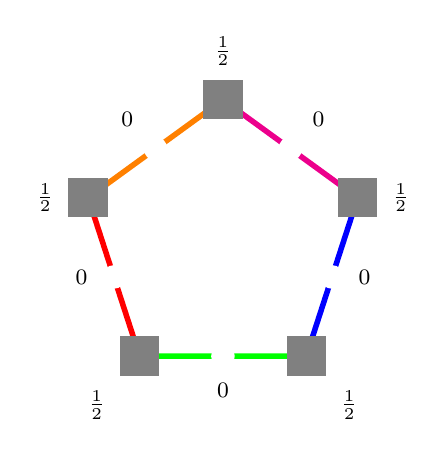
\begin{tikzpicture}  [scale=0.3]

\newdimen\ms
\ms=0.1cm

\tikzstyle{every path}=[line width=2pt]

\tikzstyle{c3}=[circle,inner sep={\ms/8},minimum size=3*\ms]
\tikzstyle{c2}=[circle,inner sep={\ms/8},minimum size=1.5*\ms]
\tikzstyle{c1}=[circle,inner sep={\ms/8},minimum size=1.1*\ms]
\tikzstyle{s1}=[rectangle,inner sep={\ms/8},minimum size=5*\ms]

% Radius of regular polygons
\newdimen\R
\R=6cm     % outer circle

%\r= { \R * sqrt(3) }     % inner circle
%\newdimen\r
%\r=    {\R * sqrt(3)/2}       % inner circle

%\newdimen\K
%\K=3cm

% Define positions of all observables
\path
  ({90 + 0 * 360 /5}:\R      ) coordinate(1)
  ({90 + 36 + 0 * 360 /5}:{\R * sqrt((25+10*sqrt(5))/(50+10*sqrt(5)))}      ) coordinate(2)
  ({90 + 1 * 360 /5}:\R   ) coordinate(3)
  ({90 + 36 + 1 * 360 /5}:{\R * sqrt((25+10*sqrt(5))/(50+10*sqrt(5)))}   ) coordinate(4)
  ({90 + 2 * 360 /5}:\R  ) coordinate(5)
  ({90 + 36 + 2 * 360 /5}:{\R * sqrt((25+10*sqrt(5))/(50+10*sqrt(5)))}  ) coordinate(6)
  ({90 + 3 * 360 /5}:\R  ) coordinate(7)
  ({90 + 36 + 3 * 360 /5}:{\R * sqrt((25+10*sqrt(5))/(50+10*sqrt(5)))}  ) coordinate(8)
  ({90 + 4 * 360 /5}:\R     ) coordinate(9)
  ({90 + 36 + 4 * 360 /5}:{\R * sqrt((25+10*sqrt(5))/(50+10*sqrt(5)))}     ) coordinate(10)
;

% draw contexts

\draw [color=orange] (1) -- (2) -- (3);
\draw [color=red] (3) -- (4) -- (5);
\draw [color=green] (5) -- (6) -- (7);
\draw [color=blue] (7) -- (8) -- (9);
\draw [color=magenta] (9) -- (10) -- (1);    %


%
%%
%% draw atoms
%%
%
\draw (1) coordinate[s1,fill=gray,label=90:{\footnotesize $\frac{1}{2}$}];   %
%
\draw (2) coordinate[c3,fill=white,label={above left:\footnotesize $0$}];    %
%
\draw (3) coordinate[s1,fill=gray,label={left:\footnotesize $\frac{1}{2}$}]; %
%
\draw (4) coordinate[c3,fill=white,label={left:\footnotesize $0$}];  %
%
\draw (5) coordinate[s1,fill=gray,label={below left:\footnotesize $\frac{1}{2}$}];  %
%
\draw (6) coordinate[c3,fill=white,label={below:\footnotesize $0$}];
%
\draw (7) coordinate[s1,fill=gray,label={below right:\footnotesize $\frac{1}{2}$}];  %
%
\draw (8) coordinate[c3,fill=white,label={right:\footnotesize $0$}];  %
%
\draw (9) coordinate[s1,fill=gray,label={right:\footnotesize $\frac{1}{2}$}];
%
\draw (10) coordinate[c3,fill=white,label={above right:\footnotesize $0$}];  %
%
%

\end{tikzpicture}
\end{center}
\end{frame}

\begin{frame}[fragile]{Examples II: Specker's ``K\"afer'' (bug) combologic (Kochen{\&}Specker, 1965, 67) - {\color{white}true (1) implies false (0)} / true (1) / inseparable logics}

\begin{center}
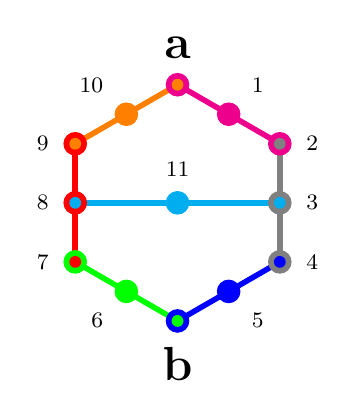
\begin{tikzpicture}  [scale=0.25]

\newdimen\ms
\ms=0.1cm

\tikzstyle{every path}=[line width=2pt]

\tikzstyle{c3}=[circle,inner sep={\ms/8},minimum size=3*\ms]
\tikzstyle{c2}=[circle,inner sep={\ms/8},minimum size=1.5*\ms]
\tikzstyle{c1}=[circle,inner sep={\ms/8},minimum size=1.1*\ms]

% Radius of regular polygons
\newdimen\R
\R=6cm     % outer circle

%\r= { \R * sqrt(3) }     % inner circle
%\newdimen\r
%\r=    {\R * sqrt(3)/2}       % inner circle

%\newdimen\K
%\K=3cm

% Define positions of all observables
\path
  ({90 + 0 * 360 /6}:\R      ) coordinate(1)
  ({90 + 30 + 0 * 360 /6}:{\R * sqrt(3)/2}      ) coordinate(2)
  ({90 + 1 * 360 /6}:\R   ) coordinate(3)
  ({90 + 30 + 1 * 360 /6}:{\R * sqrt(3)/2}   ) coordinate(4)
  ({90 + 2 * 360 /6}:\R  ) coordinate(5)
  ({90 + 30 + 2 * 360 /6}:{\R * sqrt(3)/2}  ) coordinate(6)
  ({90 + 3 * 360 /6}:\R  ) coordinate(7)
  ({90 + 30 + 3 * 360 /6}:{\R * sqrt(3)/2}  ) coordinate(8)
  ({90 + 4 * 360 /6}:\R     ) coordinate(9)
  ({90 + 30 + 4 * 360 /6}:{\R * sqrt(3)/2}     ) coordinate(10)
  ({90 + 5 * 360 /6}:\R     ) coordinate(11)
  ({90 + 30 + 5 * 360 /6}:{\R * sqrt(3)/2}     ) coordinate(12)
  (0,0) coordinate(13)
;

% draw contexts

\draw [color=orange] (1) -- (2) -- (3);
\draw [color=red] (3) -- (4) -- (5);
\draw [color=green] (5) -- (6) -- (7);
\draw [color=blue] (7) -- (8) -- (9);
\draw [color=gray] (9) -- (10) -- (11);    %
\draw [color=magenta] (11) -- (12) -- (1);    %
\draw [color=cyan] (4) -- (10);

%
%%
%% draw atoms
%%
%

\draw (1) coordinate[c3,fill=magenta,label=90:\LARGE ${\bf a}$];   %
\draw (1) coordinate[c2,fill=orange];  %
%
\draw (2) coordinate[c3,fill=orange,label=140:{\footnotesize 10}];    %
%
\draw (3) coordinate[c3,fill=red,label=180:{\footnotesize 9}]; %
\draw (3) coordinate[c2,fill=orange];  %
%
\draw (4) coordinate[c3,fill=red,label=180:{\footnotesize 8}];  %
\draw (4) coordinate[c2,fill=cyan];  %
%
\draw (5) coordinate[c3,fill=green,label=180:{\footnotesize 7}];  %
\draw (5) coordinate[c2,fill=red];  %
%
\draw (6) coordinate[c3,fill=green,label=220:{\footnotesize 6}];
%
\draw (7) coordinate[c3,fill=blue,label=270:\LARGE ${\bf b}$];  %
\draw (7) coordinate[c2,fill=green];  %
%
\draw (8) coordinate[c3,fill=blue,label=320:{\footnotesize 5}];  %
%
\draw (9) coordinate[c3,fill=gray,label=0:{\footnotesize 4}];
\draw (9) coordinate[c2,fill=blue];  %
%
\draw (10) coordinate[c3,fill=gray,label=0:{\footnotesize 3}];  %
\draw (10) coordinate[c2,fill=cyan];  %
%
\draw (11) coordinate[c3,fill=magenta,label=0:{\footnotesize 2}];  %
\draw (11) coordinate[c2,fill=gray]; %
%
\draw (12) coordinate[c3,fill=magenta,label=40:{\footnotesize 1}];  %
%
\draw (13) coordinate[c3,fill=cyan,label=90:{\footnotesize 11}];  %

\end{tikzpicture}
\end{center}
\end{frame}

\begin{frame}[fragile]{Examples II: Specker's ``K\"afer'' (bug) combologic (Kochen{\&}Specker, 1965, 67) - {\color{white} true (1) implies} false (0) / {\color{white}true (1)} / inseparable logics}

\begin{center}
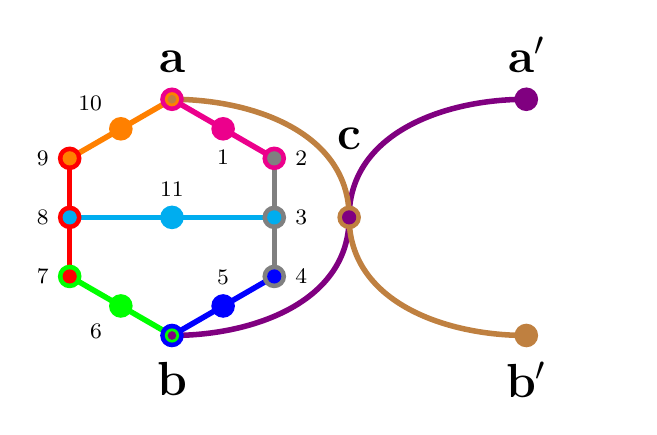
\begin{tikzpicture}  [scale=0.25]

\newdimen\ms
\ms=0.1cm

\tikzstyle{every path}=[line width=2pt]

\tikzstyle{c3}=[circle,inner sep={\ms/8},minimum size=3*\ms]
\tikzstyle{c2}=[circle,inner sep={\ms/8},minimum size=1.8*\ms]
\tikzstyle{c1}=[circle,inner sep={\ms/8},minimum size=1.1*\ms]

% Radius of regular polygons
\newdimen\R
\R=6cm     % outer circle

%\r= { \R * sqrt(3) }     % inner circle
%\newdimen\r
%\r=    {\R * sqrt(3)/2}       % inner circle

\newdimen\K
\K=18cm

% Define positions of all observables
\path
  ({90 + 0 * 360 /6}:\R      ) coordinate(1)
  ({90 + 30 + 0 * 360 /6}:{\R * sqrt(3)/2}      ) coordinate(2)
  ({90 + 1 * 360 /6}:\R   ) coordinate(3)
  ({90 + 30 + 1 * 360 /6}:{\R * sqrt(3)/2}   ) coordinate(4)
  ({90 + 2 * 360 /6}:\R  ) coordinate(5)
  ({90 + 30 + 2 * 360 /6}:{\R * sqrt(3)/2}  ) coordinate(6)
  ({90 + 3 * 360 /6}:\R  ) coordinate(7)
  ({90 + 30 + 3 * 360 /6}:{\R * sqrt(3)/2}  ) coordinate(8)
  ({90 + 4 * 360 /6}:\R     ) coordinate(9)
  ({90 + 30 + 4 * 360 /6}:{\R * sqrt(3)/2}     ) coordinate(10)
  ({90 + 5 * 360 /6}:\R     ) coordinate(11)
  ({90 + 30 + 5 * 360 /6}:{\R * sqrt(3)/2}     ) coordinate(12)
  (0,0) coordinate(13)

  ({90 + 0 * 360 /6}:\R     ) + (\K,0)  coordinate(21)
  ({90 + 30 + 0 * 360 /6}:{\R * sqrt(3)/2}     ) + (\K,0)  coordinate(22)
  ({90 + 1 * 360 /6}:\R  ) + (\K,0)  coordinate(23)
  ({90 + 30 + 1 * 360 /6}:{\R * sqrt(3)/2}  ) + (\K,0)  coordinate(24)
  ({90 + 2 * 360 /6}:\R  ) + (\K,0) coordinate(25)
  ({90 + 30 + 2 * 360 /6}:{\R * sqrt(3)/2}  ) + (\K,0)  coordinate(26)
  ({90 + 3 * 360 /6}:\R  ) + (\K,0)  coordinate(27)
  ({90 + 30 + 3 * 360 /6}:{\R * sqrt(3)/2}  ) + (\K,0)  coordinate(28)
  ({90 + 4 * 360 /6}:\R    ) + (\K,0)  coordinate(29)
  ({90 + 30 + 4 * 360 /6}:{\R * sqrt(3)/2}    ) + (\K,0)  coordinate(210)
  ({90 + 5 * 360 /6}:\R    ) + (\K,0)  coordinate(211)
  ({90 + 30 + 5 * 360 /6}:{\R * sqrt(3)/2}    ) + (\K,0)  coordinate(212)
  (0,0) + (\K,0) coordinate(213)

   (0,0) + ({\K/2},0) coordinate(40)
;

% draw contexts

\draw [color=orange] (1) -- (2) -- (3);
\draw [color=red] (3) -- (4) -- (5);
\draw [color=green] (5) -- (6) -- (7);
\draw [color=blue] (7) -- (8) -- (9);
\draw [color=gray] (9) -- (10) -- (11);    %
\draw [color=magenta] (11) -- (12) -- (1);    %
\draw [color=cyan] (4) -- (10);

\draw [color=violet] (7)  to   [out=0,in=270] (40) to [out=90,in=180] (21);
\draw [color=brown] (27)  to   [out=180,in=270] (40) to [out=90,in=0] (1);

%
%%
%% draw atoms
%%
%


\draw (1) coordinate[c3,fill=magenta,label=90:\LARGE ${\bf a}$];   %
\draw (1) coordinate[c2,fill=orange];  %
\draw (1) coordinate[c1,fill=brown];  %
%
\draw (2) coordinate[c3,fill=orange,label={[label distance=-2]140:{\footnotesize 10}}];    %
%
\draw (3) coordinate[c3,fill=red,label={[label distance=-2]180:{\footnotesize 9}}]; %
\draw (3) coordinate[c2,fill=orange];  %
%
\draw (4) coordinate[c3,fill=red,label={[label distance=-2]180:{\footnotesize 8}}];  %
\draw (4) coordinate[c2,fill=cyan];  %
%
\draw (5) coordinate[c3,fill=green,label={[label distance=-2]180:{\footnotesize 7}}];  %
\draw (5) coordinate[c2,fill=red];  %
%
\draw (6) coordinate[c3,fill=green,label={[label distance=-2]220:{\footnotesize 6}}];
%
\draw (7) coordinate[c3,fill=blue,label=270:\LARGE ${\bf b}$];  %
\draw (7) coordinate[c2,fill=green];  %
\draw (7) coordinate[c1,fill=violet];  %
%
\draw (8) coordinate[c3,fill=blue,label={[label distance=-2]90:{\footnotesize 5}}];  %
%
\draw (9) coordinate[c3,fill=gray,label={[label distance=-2]0:{\footnotesize 4}}];
\draw (9) coordinate[c2,fill=blue];  %
%
\draw (10) coordinate[c3,fill=gray,label={[label distance=-2]0:{\footnotesize 3}}];  %
\draw (10) coordinate[c2,fill=cyan];  %
%
\draw (11) coordinate[c3,fill=magenta,label={[label distance=-2]0:{\footnotesize 2}}];  %
\draw (11) coordinate[c2,fill=gray]; %
%
\draw (12) coordinate[c3,fill=magenta,label={[label distance=-2]270:{\footnotesize 1}}];  %
%
\draw (13) coordinate[c3,fill=cyan,label={[label distance=-2]90:{\footnotesize 11}}];  %



\draw (21) coordinate[c3,fill=violet,label=90:\LARGE ${\bf a}'$];   %

\draw (27) coordinate[c3,fill=brown,label=270:\LARGE ${\bf b}'$];  %



\draw (40) coordinate[c3,fill=brown,label={[label distance=15]90:\LARGE ${\bf c}$}];  %
\draw (40) coordinate[c2,fill=violet];  %

\end{tikzpicture}
\end{center}
\end{frame}

\begin{frame}[fragile]{Examples II: Specker's ``K\"afer'' (bug) combologic (Kochen{\&}Specker, 1965, 67) - {\color{white}true (1) implies} false (0) / true (1) / {\color{white}inseparable} logics}

\begin{center}
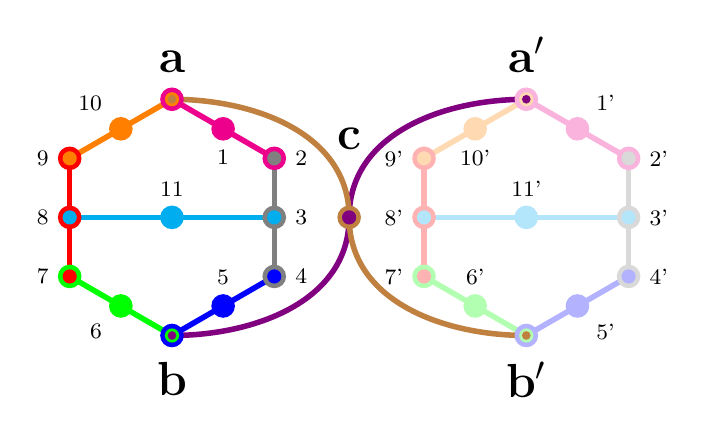
\begin{tikzpicture}  [scale=0.25]

\newdimen\ms
\ms=0.1cm

\tikzstyle{every path}=[line width=2pt]

\tikzstyle{c3}=[circle,inner sep={\ms/8},minimum size=3*\ms]
\tikzstyle{c2}=[circle,inner sep={\ms/8},minimum size=1.8*\ms]
\tikzstyle{c1}=[circle,inner sep={\ms/8},minimum size=1.1*\ms]

% Radius of regular polygons
\newdimen\R
\R=6cm     % outer circle

%\r= { \R * sqrt(3) }     % inner circle
%\newdimen\r
%\r=    {\R * sqrt(3)/2}       % inner circle

\newdimen\K
\K=18cm

% Define positions of all observables
\path
  ({90 + 0 * 360 /6}:\R      ) coordinate(1)
  ({90 + 30 + 0 * 360 /6}:{\R * sqrt(3)/2}      ) coordinate(2)
  ({90 + 1 * 360 /6}:\R   ) coordinate(3)
  ({90 + 30 + 1 * 360 /6}:{\R * sqrt(3)/2}   ) coordinate(4)
  ({90 + 2 * 360 /6}:\R  ) coordinate(5)
  ({90 + 30 + 2 * 360 /6}:{\R * sqrt(3)/2}  ) coordinate(6)
  ({90 + 3 * 360 /6}:\R  ) coordinate(7)
  ({90 + 30 + 3 * 360 /6}:{\R * sqrt(3)/2}  ) coordinate(8)
  ({90 + 4 * 360 /6}:\R     ) coordinate(9)
  ({90 + 30 + 4 * 360 /6}:{\R * sqrt(3)/2}     ) coordinate(10)
  ({90 + 5 * 360 /6}:\R     ) coordinate(11)
  ({90 + 30 + 5 * 360 /6}:{\R * sqrt(3)/2}     ) coordinate(12)
  (0,0) coordinate(13)

  ({90 + 0 * 360 /6}:\R     ) + (\K,0)  coordinate(21)
  ({90 + 30 + 0 * 360 /6}:{\R * sqrt(3)/2}     ) + (\K,0)  coordinate(22)
  ({90 + 1 * 360 /6}:\R  ) + (\K,0)  coordinate(23)
  ({90 + 30 + 1 * 360 /6}:{\R * sqrt(3)/2}  ) + (\K,0)  coordinate(24)
  ({90 + 2 * 360 /6}:\R  ) + (\K,0) coordinate(25)
  ({90 + 30 + 2 * 360 /6}:{\R * sqrt(3)/2}  ) + (\K,0)  coordinate(26)
  ({90 + 3 * 360 /6}:\R  ) + (\K,0)  coordinate(27)
  ({90 + 30 + 3 * 360 /6}:{\R * sqrt(3)/2}  ) + (\K,0)  coordinate(28)
  ({90 + 4 * 360 /6}:\R    ) + (\K,0)  coordinate(29)
  ({90 + 30 + 4 * 360 /6}:{\R * sqrt(3)/2}    ) + (\K,0)  coordinate(210)
  ({90 + 5 * 360 /6}:\R    ) + (\K,0)  coordinate(211)
  ({90 + 30 + 5 * 360 /6}:{\R * sqrt(3)/2}    ) + (\K,0)  coordinate(212)
  (0,0) + (\K,0) coordinate(213)

   (0,0) + ({\K/2},0) coordinate(40)
;

% draw contexts

\draw [color=orange] (1) -- (2) -- (3);
\draw [color=red] (3) -- (4) -- (5);
\draw [color=green] (5) -- (6) -- (7);
\draw [color=blue] (7) -- (8) -- (9);
\draw [color=gray] (9) -- (10) -- (11);    %
\draw [color=magenta] (11) -- (12) -- (1);    %
\draw [color=cyan] (4) -- (10);

\draw [color=orange!30!white] (21) -- (22) -- (23);
\draw [color=red!30!white] (23) -- (24) -- (25);
\draw [color=green!30!white] (25) -- (26) -- (27);
\draw [color=blue!30!white] (27) -- (28) -- (29);
\draw [color=gray!30!white] (29) -- (210) -- (211);    %
\draw [color=magenta!30!white] (211) -- (212) -- (21);    %
\draw [color=cyan!30!white] (24) -- (210);


\draw [color=violet] (7)  to   [out=0,in=270] (40) to [out=90,in=180] (21);
\draw [color=brown] (27)  to   [out=180,in=270] (40) to [out=90,in=0] (1);

%
%%
%% draw atoms
%%
%

\draw (1) coordinate[c3,fill=magenta,label=90:\LARGE ${\bf a}$];   %
\draw (1) coordinate[c2,fill=orange];  %
\draw (1) coordinate[c1,fill=brown];  %
%
\draw (2) coordinate[c3,fill=orange,label={[label distance=-2]140:{\footnotesize 10}}];    %
%
\draw (3) coordinate[c3,fill=red,label={[label distance=-2]180:{\footnotesize 9}}]; %
\draw (3) coordinate[c2,fill=orange];  %
%
\draw (4) coordinate[c3,fill=red,label={[label distance=-2]180:{\footnotesize 8}}];  %
\draw (4) coordinate[c2,fill=cyan];  %
%
\draw (5) coordinate[c3,fill=green,label={[label distance=-2]180:{\footnotesize 7}}];  %
\draw (5) coordinate[c2,fill=red];  %
%
\draw (6) coordinate[c3,fill=green,label={[label distance=-2]220:{\footnotesize 6}}];
%
\draw (7) coordinate[c3,fill=blue,label=270:\LARGE ${\bf b}$];  %
\draw (7) coordinate[c2,fill=green];  %
\draw (7) coordinate[c1,fill=violet];  %
%
\draw (8) coordinate[c3,fill=blue,label={[label distance=-2]90:{\footnotesize 5}}];  %
%
\draw (9) coordinate[c3,fill=gray,label={[label distance=-2]0:{\footnotesize 4}}];
\draw (9) coordinate[c2,fill=blue];  %
%
\draw (10) coordinate[c3,fill=gray,label={[label distance=-2]0:{\footnotesize 3}}];  %
\draw (10) coordinate[c2,fill=cyan];  %
%
\draw (11) coordinate[c3,fill=magenta,label={[label distance=-2]0:{\footnotesize 2}}];  %
\draw (11) coordinate[c2,fill=gray]; %
%
\draw (12) coordinate[c3,fill=magenta,label={[label distance=-2]270:{\footnotesize 1}}];  %
%
\draw (13) coordinate[c3,fill=cyan,label={[label distance=-2]90:{\footnotesize 11}}];  %



\draw (21) coordinate[c3,fill=magenta!30!white,label=90:\LARGE ${\bf a}'$];   %
\draw (21) coordinate[c2,fill=orange!30!white];  %
\draw (21) coordinate[c1,fill=violet];  %
%
\draw (22) coordinate[c3,fill=orange!30!white,label={[label distance=-2]270:{\footnotesize 10'}}];    %
%
\draw (23) coordinate[c3,fill=red!30!white,label={[label distance=-2]180:{\footnotesize 9'}}]; %
\draw (23) coordinate[c2,fill=orange!30!white];  %
%
\draw (24) coordinate[c3,fill=red!30!white,label={[label distance=-2]180:{\footnotesize 8'}}];  %
\draw (24) coordinate[c2,fill=cyan!30!white];  %
%
\draw (25) coordinate[c3,fill=green!30!white,label={[label distance=-2]180:{\footnotesize 7'}}];  %
\draw (25) coordinate[c2,fill=red!30!white];  %
%
\draw (26) coordinate[c3,fill=green!30!white,label={[label distance=-2]90:{\footnotesize 6'}}];
%
\draw (27) coordinate[c3,fill=blue!30!white,label=270:\LARGE ${\bf b}'$];  %
\draw (27) coordinate[c2,fill=green!30!white];  %
\draw (27) coordinate[c1,fill=brown];  %
%
\draw (28) coordinate[c3,fill=blue!30!white,label={[label distance=-2]320:{\footnotesize 5'}}];  %
%
\draw (29) coordinate[c3,fill=gray!30!white,label={[label distance=-2]0:{\footnotesize 4'}}];
\draw (29) coordinate[c2,fill=blue!30!white];  %
%
\draw (210) coordinate[c3,fill=gray!30!white,label={[label distance=-2]0:{\footnotesize 3'}}];  %
\draw (210) coordinate[c2,fill=cyan!30!white];  %
%
\draw (211) coordinate[c3,fill=magenta!30!white,label={[label distance=-2]0:{\footnotesize 2'}}];  %
\draw (211) coordinate[c2,fill=gray!30!white]; %
%
\draw (212) coordinate[c3,fill=magenta!30!white,label={[label distance=-2]40:{\footnotesize 1'}}];  %
%
\draw (213) coordinate[c3,fill=cyan!30!white,label={[label distance=-2]90:{\footnotesize 11'}}];  %


\draw (40) coordinate[c3,fill=brown,label={[label distance=15]90:\LARGE ${\bf c}$}];  %
\draw (40) coordinate[c2,fill=violet];  %
\end{tikzpicture}
\end{center}
\end{frame}

\begin{frame}[fragile]{Example III:  {\color{white}True (1) implies false (0)} / true (1) and value indefinite / partiality logics (Abbott, Calude, Svozil 2015, Svozil 2018)}

\newif\iflabel \labelfalse
\begin{center}
\begin{tikzpicture}  [scale=0.3]

        \tikzstyle{every path}=[line width=1.5pt]
        \tikzstyle{c1}=[color=green,circle,inner sep=2.5]
        \tikzstyle{s1}=[color=red,rectangle,inner sep=3.5]
        \tikzstyle{l1}=[draw=none,circle,minimum size=4]

        % Define positions of all observables

\draw [color=orange]   (4,0) coordinate[c1,fill,label=225:{\color{white}\LARGE ${\bf b}$}] (b) -- (13,0)     coordinate[c1,fill,label=270:{\iflabel \tiny $P_2$\fi}] (2) -- (22,0)  coordinate[s1,fill,label=315:{\iflabel \tiny $P_3$\fi}] (3);
\draw [color=blue,   ] (3) -- (26,12)  coordinate[c1,fill,pos=0.8,label=0:{\iflabel \tiny $P_{21}$\fi}] (21) coordinate[s1,fill,label=0:{\iflabel \tiny $P_{23}$\fi}] (23);
\draw [color=black] (23) -- (22,18.5) coordinate[c1,fill,pos=0.4,color=black,label=0:{\iflabel \tiny $P_{29}$\fi}] (29) coordinate[c1,fill,label=45:{\iflabel \tiny $P_5$\fi}] (5);
\draw [color=magenta,] (5)-- (13,18.5)coordinate[s1,fill,label=90:{\color{white}\LARGE ${\bf a}$}] (a) -- (4,18.5)  coordinate[c1,fill,label=135:{\iflabel \tiny $P_4$\fi}] (4);
\draw [color=CadetBlue, ] (4) -- (0,12)   coordinate[c1,fill,pos=0.6,label=180:{\iflabel \tiny $P_{10}$\fi}] (10) coordinate[s1,fill,label=180:{\iflabel \tiny $P_7$\fi}] (7);
\draw [color=brown,  ](7) -- (b)       coordinate[c1,fill,pos=0.2,label=180:{\iflabel \tiny $P_6$\fi}] (6);

        \draw [color=gray] (a) -- (2) coordinate[c1,fill,pos=0.5,label=315:{\iflabel \tiny $P_1$\fi}] (1);

        \draw [color=violet] (5) -- (22,6) coordinate[s1,fill,pos=0.4,label=0:{\iflabel \tiny $P_{11}$\fi}] (11) coordinate[c1,fill,label=0:{\iflabel \tiny $P_9$\fi}] (9);

\draw [color=Apricot] (9) -- (b) coordinate[s1,fill,pos=0.3,label=280:{\iflabel \tiny $P_8$\fi}] (8);

\draw [color=TealBlue] (4) -- (4,6) coordinate[s1,fill,pos=0.4,label=180:{\iflabel \tiny $P_{28}$\fi}] (28) coordinate[c1,fill,label=180:{\iflabel \tiny $P_{22}$\fi}] (22);
\draw [color=YellowGreen] (22) -- (3) coordinate[c1,fill,pos=0.2,label=260:{\iflabel \tiny $P_{19}$\fi}] (19);

        \coordinate (25) at ([xshift=-4cm]1);
        \coordinate (27) at ([xshift=4cm]1);

\draw [color=MidnightBlue]  (22) -- (25) coordinate[c1,fill,pos=0.5,label=115:{\iflabel \tiny $P_{24}$\fi}] (24) coordinate[s1,fill,label=270:{\iflabel \tiny $P_{25}$\fi}] (25);
\draw [color=Mulberry] (25) -- (9) coordinate[c1,fill,pos=0.8,label=90:{\iflabel \tiny $P_{35}$\fi}] (35);

\draw [color=BrickRed]  (7) -- (27) coordinate[c1,fill,pos=0.5,label=90:{\iflabel \tiny $P_{34}$\fi}] (34) coordinate[c1,fill,label=90:{\iflabel \tiny $P_{27}$\fi}] (27);
\draw [color=Emerald] (27) -- (23) coordinate[c1,fill,pos=0.25,label=270:{\iflabel \tiny $P_{26}$\fi}] (26);

\draw [color=BlueGreen]  (10) -- (15.5,17.5) coordinate[c1,fill,pos=0.5,label=90:{\iflabel \tiny $P_{12}$\fi}] (12) coordinate[s1,fill,label=15:{\iflabel \tiny $P_{13}$\fi}] (13);
%\draw [color=Tan] (13) -- (29) coordinate[c1,fill,pos=0.4,label=90:{\iflabel \tiny $P_{31}$\fi}] (31);

\draw [color=RawSienna]  (28) -- (10.5,15) coordinate[c1,fill,pos=0.5,label=90:{\iflabel \tiny $P_{30}$\fi}] (30) coordinate[c1,fill,label=90:{\iflabel \tiny $P_{15}$\fi}] (15);
\draw [color=SpringGreen] (15) -- (11) coordinate[c1,fill,pos=0.6,label=90:{\iflabel \tiny $P_{14}$\fi}] (14);

\draw [color=Salmon]  (15) -- (1) coordinate[s1,fill,pos=0.2,label=15:{\iflabel \tiny $P_{17}$\fi}] (17);
\draw [color=Fuchsia] (1)-- (13) coordinate[c1,fill,pos=0.3,label=0:{\iflabel \tiny $P_{16}$\fi}] (16);

\draw [color=CornflowerBlue]  (19) -- (16) coordinate[s1,fill,pos=0.3,label=180:{\iflabel \tiny $P_{18}$\fi}] (18);
\draw [color=pink] (16) -- (8) coordinate[c1,fill,pos=0.7,label=180:{\iflabel \tiny $P_{32}$\fi}] (32);

\draw [color=PineGreen]  (6) -- (17) coordinate[c1,fill,pos=0.7,label=90:{\iflabel \tiny $P_{33}$\fi}] (33);
\draw [color=DarkOrchid] (17) -- (21) coordinate[c1,fill,pos=0.4,label=90:{\iflabel \tiny $P_{20}$\fi}] (20);

\draw [color=black] (25)  -- (1) -- (27);

%\coordinate (ContextLabel) at ([shift=({-2cm,-3mm})]1);
%\draw (ContextLabel) coordinate[l1,label=90:{\iflabel \tiny $C_{26}$\fi}];

\end{tikzpicture}
\end{center}
\end{frame}

\begin{frame}[fragile]{Example III:  {\color{white}True (1) implies} false (0) / {\color{white}true (1)} and value indefinite / partiality logics (Abbott, Calude, Svozil 2015, Svozil 2018)}

\newif\iflabel \labelfalse
\begin{center}
\begin{tikzpicture}  [scale=0.3]

        \tikzstyle{every path}=[line width=1.5pt]
        \tikzstyle{c1}=[color=green,circle,inner sep=2.5]
        \tikzstyle{s1}=[color=red,rectangle,inner sep=3.5]
        \tikzstyle{l1}=[draw=none,circle,minimum size=4]

        % Define positions of all observables

\draw [color=orange]   (4,0) coordinate[s1,fill,label=225:{\color{white}\LARGE ${\bf b}$}] (b) -- (13,0)     coordinate[c1,fill,label=270:{\iflabel \tiny $P_2$\fi}] (2) -- (22,0)  coordinate[c1,fill,label=315:{\iflabel \tiny $P_3$\fi}] (3);
\draw [color=blue,   ] (3) -- (26,12)  coordinate[c1,fill,pos=0.8,label=0:{\iflabel \tiny $P_{21}$\fi}] (21) coordinate[s1,fill,label=0:{\iflabel \tiny $P_{23}$\fi}] (23);
\draw [color=green] (23) -- (22,18.5) coordinate[c1,fill,pos=0.4,label=0:{\iflabel \tiny $P_{29}$\fi}] (29) coordinate[c1,fill,label=45:{\iflabel \tiny $P_5$\fi}] (5);
\draw [color=magenta,] (5)-- (13,18.5)coordinate[s1,fill,label=90:{\color{white}\LARGE ${\bf a}$}] (a) -- (4,18.5)  coordinate[c1,fill,label=135:{\iflabel \tiny $P_4$\fi}] (4);
\draw [color=black] (4) -- (0,12)   coordinate[c1,color=black,fill,pos=0.6,label=180:{\iflabel \tiny $P_{10}$\fi}] (10) coordinate[c1,fill,label=180:{\iflabel \tiny $P_7$\fi}] (7);
\draw [color=brown,  ] (7) -- (b)      coordinate[c1,fill,pos=0.2,label=180:{\iflabel \tiny $P_6$\fi}] (6);

        \draw [color=gray] (a) -- (2) coordinate[c1,fill,pos=0.5,label=315:{\iflabel \tiny $P_1$\fi}] (1);

        \draw [color=violet] (5) -- (22,6) coordinate[s1,fill,pos=0.4,label=0:{\iflabel \tiny $P_{11}$\fi}] (11) coordinate[c1,fill,label=0:{\iflabel \tiny $P_9$\fi}] (9);

\draw [color=Apricot] (9) -- (b) coordinate[c1,fill,pos=0.3,label=280:{\iflabel \tiny $P_8$\fi}] (8);

\draw [color=TealBlue] (4) -- (4,6) coordinate[s1,fill,pos=0.4,label=180:{\iflabel \tiny $P_{28}$\fi}] (28) coordinate[c1,fill,label=180:{\iflabel \tiny $P_{22}$\fi}] (22);
\draw [color=YellowGreen] (22) -- (3) coordinate[s1,fill,pos=0.2,label=260:{\iflabel \tiny $P_{19}$\fi}] (19);

        \coordinate (25) at ([xshift=-4cm]1);
        \coordinate (27) at ([xshift=4cm]1);

\draw [color=MidnightBlue]  (22) -- (25) coordinate[c1,fill,pos=0.5,label=115:{\iflabel \tiny $P_{24}$\fi}] (24) coordinate[s1,fill,label=270:{\iflabel \tiny $P_{25}$\fi}] (25);
\draw [color=Mulberry] (25) -- (9) coordinate[s1,fill,pos=0.8,label=90:{\iflabel \tiny $P_{35}$\fi}] (35);

\draw [color=BrickRed]  (7) -- (27) coordinate[c1,fill,pos=0.5,label=90:{\iflabel \tiny $P_{34}$\fi}] (34) coordinate[c1,fill,label=90:{\iflabel \tiny $P_{27}$\fi}] (27);
\draw [color=Emerald] (27) -- (23) coordinate[c1,fill,pos=0.25,label=270:{\iflabel \tiny $P_{26}$\fi}] (26);

\draw [color=black]  (10) -- (15.5,17.5) coordinate[c1,color=black,fill,pos=0.5,label=90:{\iflabel \tiny $P_{12}$\fi}] (12) coordinate[s1,fill,label=15:{\iflabel \tiny $P_{13}$\fi}] (13);
\draw [color=Tan] (13) -- (29) coordinate[c1,fill,pos=0.4,label=90:{\iflabel \tiny $P_{31}$\fi}] (31);

\draw [color=RawSienna]  (28) -- (10.5,15) coordinate[c1,fill,pos=0.5,label=90:{\iflabel \tiny $P_{30}$\fi}] (30) coordinate[c1,fill,label=90:{\iflabel \tiny $P_{15}$\fi}] (15);
\draw [color=SpringGreen] (15) -- (11) coordinate[c1,fill,pos=0.6,label=90:{\iflabel \tiny $P_{14}$\fi}] (14);

\draw [color=Salmon]  (15) -- (1) coordinate[s1,fill,pos=0.2,label=15:{\iflabel \tiny $P_{17}$\fi}] (17);
\draw [color=Fuchsia] (1)-- (13) coordinate[c1,fill,pos=0.3,label=0:{\iflabel \tiny $P_{16}$\fi}] (16);

\draw [color=CornflowerBlue]  (19) -- (16) coordinate[c1,fill,pos=0.3,label=180:{\iflabel \tiny $P_{18}$\fi}] (18);
\draw [color=pink] (16) -- (8) coordinate[s1,fill,pos=0.7,label=180:{\iflabel \tiny $P_{32}$\fi}] (32);

\draw [color=PineGreen]  (6) -- (17) coordinate[c1,fill,pos=0.7,label=90:{\iflabel \tiny $P_{33}$\fi}] (33);
\draw [color=DarkOrchid] (17) -- (21) coordinate[c1,fill,pos=0.4,label=90:{\iflabel \tiny $P_{20}$\fi}] (20);

\draw [color=black] (25) -- (1) -- (27);

        \coordinate (ContextLabel) at ([shift=({-2cm,-3mm})]1);
        \draw (ContextLabel) coordinate[l1,label=90:{\iflabel \tiny $C_{26}$\fi}];

        \end{tikzpicture}
\end{center}
\end{frame}

\begin{frame}[fragile]{Example III:  {\color{white}True (1) implies} false (0) / true (1) and {\color{white}value indefinite / partiality}  logics (Abbott, Calude, Svozil 2015, Svozil 2018)}

\newif\iflabel \labeltrue
\begin{center}
\begin{tikzpicture}  [scale=0.3]
\labeltrue
        \tikzstyle{every path}=[line width=1.5pt]
%\tikzstyle{c1}=[circle,fill,inner sep=4]
%\tikzstyle{c2}=[circle,fill,inner sep=2.7]
%\tikzstyle{c3}=[circle,fill,inner sep=1]
        \tikzstyle{c1}=[circle,fill,inner sep=3]
        \tikzstyle{c2}=[circle,fill,inner sep=2]
        \tikzstyle{c3}=[circle,fill,inner sep=1]
        \tikzstyle{s1}=[color=red,rectangle,minimum size=8,inner sep=6]
        \tikzstyle{d1}=[draw=none,circle,minimum size=4]
        \tikzstyle{e1}=[color=gray,rectangle,minimum size=8,inner sep=6]

        % Define positions of all observables



\draw [color=orange]  (4,0)  coordinate[c1,fill,label=225:{\color{white}\LARGE ${\bf b}$}] (b) -- (13,0)    coordinate[c1,fill,label={[label distance=-1]270:{\iflabel \footnotesize \color{white}  $2$\fi}}] (2) -- (22,0)  coordinate[c1,fill,label={[label distance=-1]315:{\iflabel \footnotesize \color{white}  $3$\fi}}] (3);
\draw [color=blue] (3) -- (26,12)  coordinate[c1,fill,pos=0.8,label={[label distance=-1]0:{\iflabel \footnotesize \color{white}  ${21}$\fi}}] (21) coordinate[c1,fill,label={[label distance=-3]0:{\iflabel \footnotesize \color{white}  ${23}$\fi}}] (23);
\draw [color=green] (23) -- (22,18.5) coordinate[c1,fill,pos=0.4,label={[label distance=-1]0:{\iflabel \footnotesize \color{white}  ${29}$\fi}}] (29) coordinate[c1,fill,label={[label distance=-1]45:{\iflabel \footnotesize \color{white}  $5$\fi}}] (5);
\draw [color=magenta] (5)-- (13,18.5)coordinate[c1,fill,label=90:{\color{white}\LARGE ${\bf a}$}] (a) -- (4,18.5)  coordinate[c1,fill,label={[label distance=-1]135:{\iflabel \footnotesize \color{white}  $4$\fi}}] (4);
\draw [color=CadetBlue] (4) -- (0,12)   coordinate[c1,fill,pos=0.6,label={[label distance=-1]180:{\iflabel \footnotesize \color{white}  ${10}$\fi}}] (10)  coordinate[c1,fill,label={[label distance=-1]180:{\iflabel \footnotesize \color{white}  $7$\fi}}] (7);
\draw [color=brown] (7) -- (b)      coordinate[c1,fill,pos=0.2,label={[label distance=-1]180:{\iflabel \footnotesize \color{white}  $6$\fi}}] (6);






        \draw [color=gray] (a) -- (2) coordinate[c1,fill,pos=0.52,label={[label distance=-1, yshift=2]357.5:{\iflabel \footnotesize \color{white}  $1$\fi}}] (1);

        \draw [color=violet] (5) -- (22,6) coordinate[c1,fill,pos=0.4,label={[label distance=-1]0:{\iflabel \footnotesize \color{white}  ${11}$\fi}}] (11) coordinate[c1,fill,label={[label distance=-1]0:{\iflabel \footnotesize \color{white}  $9$\fi}}] (9);

\draw [color=Apricot] (9) -- (b) coordinate[c1,fill,pos=0.3,label={[label distance=-1]280:{\iflabel \footnotesize \color{white}  $8$\fi}}] (8);

\draw [color=TealBlue] (4) -- (4,6) coordinate[c1,fill,pos=0.4,label={[label distance=-1]180:{\iflabel \footnotesize \color{white}  ${28}$\fi}}] (28) coordinate[c1,fill,label={[label distance=-3]180:{\iflabel \footnotesize \color{white}  ${22}$\fi}}] (22);
\draw [color=YellowGreen] (22) -- (3) coordinate[c1,fill,pos=0.2,label={[label distance=-1]260:{\iflabel \footnotesize \color{white}  ${19}$\fi}}] (19);

        \coordinate (25) at ([xshift=-4cm]1);
        \coordinate (27) at ([xshift=4cm]1);

\draw [color=MidnightBlue]  (22) -- (25) coordinate[c1,fill,pos=0.5,label={[label distance=-1]180:{\iflabel \footnotesize \color{white}  ${24}$\fi}}] (24) coordinate[c1,fill,label={[label distance=-1]180:{\iflabel \footnotesize \color{white}  ${25}$\fi}}] (25);
\draw [color=Mulberry] (25) -- (9) coordinate[c1,fill,pos=0.8,label={[label distance=-1]90:{\iflabel \footnotesize \color{white}  ${35}$\fi}}] (35);

\draw [color=BrickRed]  (7) -- (27) coordinate[c1,fill,pos=0.5,label={[label distance=-3]90:{\iflabel \footnotesize \color{white}  ${34}$\fi}}] (34) coordinate[c1,fill,label={[label distance=-1]90:{\iflabel \footnotesize \color{white}  ${27}$\fi}}] (27);
\draw [color=Emerald] (27) -- (23) coordinate[c1,fill,pos=0.25,label={[label distance=-1]320:{\iflabel \footnotesize \color{white}  ${26}$\fi}}] (26);

\draw [color=BlueGreen]  (10) -- (15.5,17.5) coordinate[c1,fill,pos=0.5,label={[label distance=-1]90:{\iflabel \footnotesize \color{white}  ${12}$\fi}}] (12) coordinate[c1,fill,label={[label distance=-1,xshift=5]270:{\iflabel \footnotesize \color{white}  ${13}$\fi}}] (13);
\draw [color=Tan] (13) -- (29) coordinate[c1,fill,pos=0.4,label={[label distance=-1]90:{\iflabel \footnotesize \color{white}  ${31}$\fi}}] (31);

\draw [color=RawSienna]  (28) -- (10.5,15) coordinate[c1,fill,pos=0.5,label={[label distance=-3, yshift=-3]160:{\iflabel \footnotesize \color{white}  ${30}$\fi}}] (30) coordinate[c1,fill,label={[label distance=-5]45:{\iflabel \footnotesize \color{white}  ${15}$\fi}}] (15);
\draw [color=SpringGreen] (15) -- (11) coordinate[c1,fill,pos=0.6,label={[label distance=-1]90:{\iflabel \footnotesize \color{white}  ${14}$\fi}}] (14);

\draw [color=Salmon]  (15) -- (1) coordinate[c1,fill,pos=0.2,label={[label distance=-1, yshift=2]180:{\iflabel \footnotesize \color{white}  ${17}$\fi}}] (17);
\draw [color=Fuchsia] (1)-- (13) coordinate[c1,fill,pos=0.3,label={[label distance=-1]0:{\iflabel \footnotesize \color{white}  ${16}$\fi}}] (16);

\draw [color=CornflowerBlue]  (19) -- (16) coordinate[c1,fill,pos=0.3,label={[label distance=-1]180:{\iflabel \footnotesize \color{white}  ${18}$\fi}}] (18);
\draw [color=pink] (16) -- (8) coordinate[c1,fill,pos=0.7,label={[label distance=-1]180:{\iflabel \footnotesize \color{white}  ${32}$\fi}}] (32);

\draw [color=PineGreen]  (6) -- (17) coordinate[c1,fill,pos=0.7,label={[label distance=-1, yshift=2]180:{\iflabel \footnotesize \color{white}  ${33}$\fi}}] (33);
\draw [color=DarkOrchid] (17) -- (21) coordinate[c1,fill,pos=0.4,label={[label distance=-3]20:{\iflabel \footnotesize \color{white}  ${20}$\fi}}] (20);

\draw [color=black] (25) -- (1) -- (27);




\draw (a) coordinate[c2,fill=gray];

\draw (b) coordinate[c2,fill=brown];
\draw (b) coordinate[c3,fill=Apricot];

\draw (4) coordinate[c2,fill=CadetBlue];
\draw (4) coordinate[c3,fill=TealBlue];

\draw (5) coordinate[c2,fill=magenta];
\draw (5) coordinate[c3,fill=violet];

\draw (7) coordinate[c2,BrickRed];
\draw (7) coordinate[c3,fill=brown];

\draw (23) coordinate[c2,fill=green];
\draw (23) coordinate[c3,fill=Emerald];

\draw (29) coordinate[c2,fill=Tan];

\draw (21) coordinate[c2,fill=DarkOrchid];

\draw (3) coordinate[c2,fill=blue];
\draw (3) coordinate[c3,fill=YellowGreen];

\draw (11) coordinate[c2,fill=SpringGreen];

\draw (9) coordinate[c2,fill=Apricot];
\draw (9) coordinate[c3,fill=Mulberry];

\draw (27) coordinate[c2,fill=Emerald];
\draw (27) coordinate[c3,fill=black];

\draw (13) coordinate[c2,fill=Tan];
\draw (13) coordinate[c3,fill=Fuchsia];

\draw (7) coordinate[c2,BrickRed];
\draw (7) coordinate[c3,fill=brown];

\draw (8) coordinate[c2,fill=pink];

\draw (19) coordinate[c2,fill=CornflowerBlue];

\draw (16) coordinate[c2,fill=CornflowerBlue];
\draw (16) coordinate[c3,fill=pink];

\draw (1) coordinate[c2,fill=Salmon];
\draw (1) coordinate[c3,fill=Fuchsia];

\draw (17) coordinate[c2,fill=PineGreen];
\draw (17) coordinate[c3,fill=DarkOrchid];

\draw (15) coordinate[c2,fill=SpringGreen];
\draw (15) coordinate[c3,fill=Salmon];

\draw (25) coordinate[c2,fill=Mulberry];
\draw (25) coordinate[c3,fill=black];


\draw (22) coordinate[c2,fill=YellowGreen];
\draw (22) coordinate[c3,fill=MidnightBlue];

\draw (28) coordinate[c2,fill=RawSienna];

\draw (10) coordinate[c2,fill=BlueGreen];

\draw (6) coordinate[c2,fill=PineGreen];


\draw (2) coordinate[c2,fill=gray];

\end{tikzpicture}
 \end{center}
\end{frame}


\begin{frame}[fragile]{Strategies to obtain  value indefiniteness / partiality}

The scheme of the construction \& proof of partiality of value assignments is as follows:
\begin{itemize}
\item[(i)]
Find a logic (collection of intertwined contexts of observables) exhibiting a true-implies-false  property on the two atoms ${\bf a}$ and ${\bf b}$.
\item[(ii)]
Find another logic exhibiting a true-implies-true property on the same two atoms ${\bf a}$ and ${\bf b}$.
\item[(iii)]
Then join (paste) these logics into a larger logic, which, given ${\bf a}$,
neither allows ${\bf b}$ to be true nor false. Consequently  ${\bf b}$ must be value indefinite.
\end{itemize}

{ \color{yellow}
ps: the Abbott, Calude, Svozil 2015 logic introduced earlier has a quantum (Hilbert space) realization of
$\vert {\bf a} \rangle = \begin{pmatrix}   1,0,0 \end{pmatrix}^\intercal$,
and
$\vert {\bf b} \rangle = \begin{pmatrix}   \frac{1}{\sqrt{2}},\frac{1}{2},\frac{1}{2} \end{pmatrix}^\intercal$;
Thus the probability to observe  ${\bf b}$ given ${\bf a} $ is 50:50.

pps: partiality /value indefiniteness /strong contextuality can be extended to {\color{red}any} vector non-collinear and non-orthogonal to ${\bf a}$.
}

\end{frame}

\begin{frame}[fragile]{Meaning of value indefiniteness/partiality of the truth assignments in view of the arbitrariness in the choice of logics connecting ${\bf a}$ and ${\bf b}$}

Given ${\bf a}$, there exist a continuum of possible pathways to ${\bf b}$; many with very different ``contextual'' properties.

Since the selection of these pathways (or logics connecting them) is merely hypothetical, personal and thus epistemic,
``I am inclined to believe'' (cf. Born 1926) that in the quantum world there does not exist an observable ${\bf b}$, given ${\bf a}$,
unless both are orthogonal or collinear. What we effectively do when we allegedly ``measure   ${\bf b}$'' are just ``translations'' of properties
which are relational (via entanglement throuh interaction) to ${\bf a}$,
mediated through our measurement devices; thereby we fapp introduce stochasticity
because of the many uncontrollable degrees of freedom of the latter.

Cf. https://arxiv.org/abs/1804.10030

\end{frame}


\frame{

\centerline{\huge {\color{yellow} Thank you for your attention!}}

\begin{center}\color{orange}
$\widetilde{\qquad \qquad }$
$\widetilde{\qquad \qquad}$
$\widetilde{\qquad \qquad }$
\end{center}
 }
 \end{document}





\begin{frame}[fragile]{Example I}

\begin{center}

\end{center}

\end{frame}

 \frame{
 \frametitle{}

 }


